\begin{frame}{Merge REU Work into Production AWS Branch}
    \begin{itemize}
        \item Aaryan's Inference Work
        \item Rahual's MongoDB Work
    \end{itemize}   
\end{frame}

\begin{frame}{Implement MongoDB Networking}
    \centering
    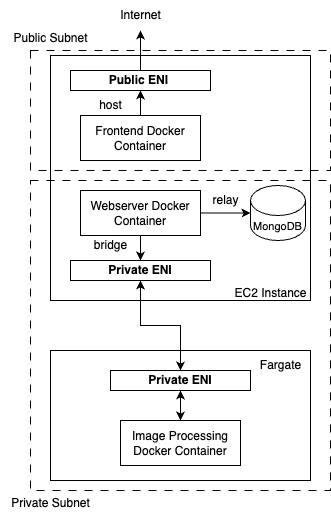
\includegraphics[height=0.8\textheight,width=0.8\textwidth,keepaspectratio]{images/mm_networking.png}
\end{frame}

\begin{frame}{Assess Maintenance Steps}
    \begin{itemize}
        \item Spin up/down infrastructure
        \item Implement on Terraform
    \end{itemize}  
\end{frame}

\begin{frame}{Test CI/CD Pipeline}
    \begin{itemize}
        \item Test Github Action for ECR Upload
        \item Test ECR Upload to ECS Service Redeploy
    \end{itemize}  
\end{frame}

\begin{frame}{Next Steps}
    \begin{itemize}
        \item NIR/SWIR
        \item Satellite Super Resolution
        \item Compare Inference Performance on Drone Datasets
    \end{itemize}  
\end{frame}


% Slides for 2024-09-30
% To create a slide, use the following:
% \begin{frame}{TITLE}
%     BODY
% \end{frame}

% To create a slide with a bullet list, use the following:
% \begin{frame}{TITLE}
%     \begin{itemize}
%         \item ITEM 1
%         \item ITEM 2
%     \end{itemize}    
% \end{frame}

% To create a slide with numbered list, use the following:
% \begin{frame}{TITLE}
%     \begin{enumerate}
%         \item ITEM 1
%         \item ITEM 2
%     \end{enumerate}
% \end{frame}

% To create a slide with a graphic:
% 1. Add the graphic to this folder (named picture.png)
% 2. Use the following:
% \begin{frame}{TITLE}
%     \centering
%     \includegraphics[height=0.7\textheight,width=0.7\textwidth,keepaspectratio]{picture.png}
% \end{frame}

% To create a slide with two columns, use the following:
% \begin{frame}{TITLE}
%     \begin{columns}
%         \begin{column}{0.5\textwidth}
%             COLUMN 1 BODY
%         \end{column}
%         \begin{column}{0.5\textwidth}
%             COLUMN 2 BODY
%         \end{column}
%     \end{columns}
% \end{frame}
